% brainstorm:

% * revisão das teorias de contornos
% * parte da análise que fiz do opus 5 mov 3 de Webern
% * exemplos de usos de operações na peça do mestrado e experimentos
% * desenvolvimento do goiaba (para que serve e um exemplo da saída)

\section{Introduction}
\label{sec:introduction}

Contours can be understood as the shape or format of an object. In
Music, contour can be associated to pitch, density, rhythm, intensity,
etc, and represents a parameter in function of another, as pitch in
function of time. For instance, Beethoven's Fifth Symphony main motive
and its contour are represented respectively in figures
\ref{fig:5a-sinfonia-motivo} and \ref{fig:c-3120}.

Contour study is important because, like motives and pitch sets,
contours can help to give coherence to a musical piece. They represent
handling musical structures through operations like inversion and
retrogradation, and can be aproached by analytical or compositional
points of view.

Despite the possible coherence given by contours and the operations
provided by contour theories (see section \ref{sec:contour-theories}),
systematic studies of contour operations and combinations usage in
musical composition are scarce. So experimentation and studies about
these operations usage in composition area are required.

In this paper we present partial results of our research about contour
applications in music composition. The first author of this paper, in
his master's\footnote{The reference was omitted to keep anonymity. It
  will be included in final version.}, composed two experimental short
pieces and an eleven minutes quintet, both based in contour theories
operations (see section \ref{sec:contour-theories}). We also have
developed a contour processor software\footnote{Additional information
  and link were also omitted to keep anonymity.}. This software
receives as input symbollic contours and outputs symbollic and
graphical representations of contours and operations.

\section{Contour theories}
\label{sec:contour-theories}

Many authors
\cite{friedmann85:methodology,friedmann87:response,morris87:composition,morris93:directions,marvin.ea87:relating,marvin88:generalized,marvin.ea95:generalization,polansky.ea92:possible,quinn97:fuzzy,clifford95:contour,beard03:contour}
have developed theories to system the contour study. These theories
were developed primarily as analytic techniques for non-tonal
compositions without typical musical features used to demonstrate
coherence in tonal compositions, like phrase, periods, themes and
functional analysis \cite{beard03:contour}.

According to these theories, absolute value of the contour elements
are ignored, and only the high-low relation between these elements is
regarded.  These theories provide arrays, matrixes and many operations
to help in comparing contours, like inversion, translation, contour
elements comparison, and contour similarity comparisons, comparison
matrix and contour interval array.

Music analysis under contour point of view have been effective in
tonal and non-tonal music. There are successful analysis of A.
Schoenberg \cite{friedmann85:methodology}, A. Webern
\cite{clifford95:contour}, L. Dallapicolla
\cite{marvin88:generalized}, and W. A. Mozart \cite{beard03:contour}
pieces. Clifford \cite{clifford95:contour}, for example, says contour
has a significant role in Webern pre-serial music structure.

\section{Contour in Composition}
\label{sec:contour-composition}

Contour can represent significant structures in compositional process
of a piece, however, studies involving systematic contour usage in
composition are scarce. Hence we began a research in which we composed
contour based experimental pieces.

This research most important result is first author's master's
thesis. In this thesis a woodwind quintet eleven minutes piece was
composed using combinations of contour operations associated with
parameters such as pitch, tempo, density and texture.

This quintet is based on a six notes motive called $\alpha$
(fig. \ref{fig:motivo-alfa})---based on octatonic scale---and its
derived contour P(5 3 4 1 2 0) (fig. \ref{fig:c-534120}). This P
contour, its subsets and operations---retrogradation, inversion,
rotation, interpollation---were the only used in the piece.

For instance, the tempo in this quintet---82, 66, 120, 108 and
112---have relations based in A(1 0 4 2 3) contour, a five elements P
subset. The number of instruments in piece first section also are
based in a P subset contour, N(1 3 2 5 4). The piece begins with a
solo, then a trio, a duo, a quintet, and finally a quartet.

In the quintet contour operations were also combined to produce new
stuff. Rotation were combinated with retrogradation, intervallic
expansion with interpolation, rotation with intervallic expansion, and
so on.

In a \eng{fugato}, in the quintet, subject and countersubject are based
on rotation and retrogradation operations. The subject has original
contour P(5 3 4 1 2 0) and factor 3 rotation
(fig. \ref{fig:sujeito-fugato}). The contoursubject has original
contour retrogradation repeated three times with different rotation
factors---5, 4 and 3 (fig. \ref{fig:contra-sujeito-fugato}).

Rotation and intervallic expansion occur like in figure
\ref{fig:notas-curtas-madeiras}. In flute the contour has original
form, and in clarinet there is a factor 2 rotation and an
expansion. In oboe there is a factor 3 rotation and contour deviation
justified by the gesture. In bassoon there is a factor 3 contour
rotation and retrogradation, and intervallic expansion.

\section{Conclusions}
\label{sec:conclusions}

Contour represented a significant structure in cited quintet
compositional process. The majority structures of the piece were
composed based in contour operations. For this reason we believe
contour is important to composition in addition to analysis. We
continue the research and have some questions to approach. For
example, contours can be used in multiple layers, associating, at the
same time pitch, duration, timbre, and dynamics, each of them in a
different layer.

The cited software has an important role in our research. Contour can
be easily recognized from graphic representation (as in figures
\ref{fig:rot-0}, \ref{fig:rot-2}, \ref{fig:rot-3}, and
\ref{fig:rot-3-retr}). Also, contour operations requires precise
mathematical handling. This software automates both tasks avoiding
human errors and loosing time. In future the software will receive as
input Lilypond\footnote{\url{http://lilypond.org/}} format scores and
will have a graphical interface.

The next steps in our research are to develop the software to provide
a better interaction with the user, and to compose short experiments
to test a larger operations corpus, and multiple layers contours.

\break
%%% concentra figuras em um só lugar

\begin{figure}[!p]
  \centering
  \subfloat[Main motive]{
    \includegraphics{5a-sinfonia}
    \label{fig:5a-sinfonia-motivo}
  }
  \subfloat[Contour (3 1 2 0)]{
    \includegraphics{c-3120}
    \label{fig:c-3120}
  }
  \caption{Fifth Symphony main motive contour}
  \label{fig:5a-sinfonia}
\end{figure}

\begin{figure}[!p]
  \centering
  \subfloat[$\alpha$ motive]{
    \includegraphics{motivo-alfa}
    \label{fig:motivo-alfa}
  }
  \subfloat[P(5 3 4 1 2 0) contour]{
    \includegraphics{c-534120}
    \label{fig:c-534120}
  }
  \caption{Materials}
  \label{fig:materials}
\end{figure}

\begin{figure}
  \centering
  \subfloat[Subject]{
    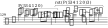
\includegraphics[scale=3.2]{sujeito-fugato}
    \label{fig:sujeito-fugato}
  }

  \subfloat[Countersubject]{
    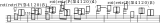
\includegraphics[scale=3.2]{contra-sujeito-fugato}
    \label{fig:contra-sujeito-fugato}
  }
  \caption{Structural elements of \eng{fugato}}
  \label{fig:elementos-fugato}
\end{figure}

\begin{figure}[!p]
  \centering
  \subfloat[4 fragments composed by rotation and expansion]{
    \includegraphics[scale=1]{notas-curtas-madeiras}
    \label{fig:notas-curtas-madeiras}
  }

  \subfloat[original]{
    \includegraphics[scale=.75]{c-534120}
    \label{fig:rot-0}
  }
  \subfloat[rot 2]{
    \includegraphics[scale=.75]{c-412053}
    \label{fig:rot-2}
  }
  \subfloat[rot 3]{
    \includegraphics[scale=.75]{c-120534}
    \label{fig:rot-3}
  }
  \subfloat[retr(rot 3)]{
    \includegraphics[scale=.75]{c-435021}
    \label{fig:rot-3-retr}
  }
  \caption{Rotation and expansion}
  \label{fig:rotacao-expansao}
\end{figure}

%%% Local Variables: 
%%% mode: latex
%%% TeX-master: "contour-composition"
%%% End: 